% !TeX root = RJwrapper.tex
\title{Spatial disaggregation modeling with R-INLA for air pollution applications}


\author{by Fernando Rodriguez Avellaneda and Paula Moraga}

\maketitle

\abstract{%
Spatial data are often available at aggregated scales due to sampling costs or privacy constraints, as commonly seen in air pollution information. This limits the ability to detect fine-scale spatial patterns that are important for environmental assessment and policy. Spatial disaggregation methods address this issue by recovering high-resolution fields from aggregated observations. A common modelling approach for spatial disaggregation assumes an underlying latent Gaussian field representing the true continuous process, linked to aggregated observations via an observation model. Bayesian inference provides a natural framework for fitting these models, but standard Markov chain Monte Carlo (MCMC) methods can be computationally demanding. As an efficient alternative, the stochastic partial differential equation (SPDE) and integrated nested Laplace approximations (INLA) approaches offer accurate and fast approximate inference.
}

\nocite{R-patchwork,R-ggplot2,R-viridis,R-kableExtra,R-terra,R-rnaturalearth,R-sf,R-tidyterra,R-fmesher,R-INLA,R-exactextractr}

\section{Introduction}\label{introduction}

Spatial data are common in fields such as environmental science, epidemiology, and ecology, but are often available in aggregated form due to reporting practices and privacy constraints For example, disease cases may be reported at administrative levels, and environmental indicators such as air pollution levels are often averaged over coarser regions. While such aggregated data are widely used and often necessary for practical and ethical reasons, they can mask fine-scale spatial variation that is important for scientific analysis and decision-making.

Spatial disaggregation methods aim to address this limitation by recovering local patterns from aggregated observations. A common modeling approach for spatial disaggregation assumes an underlying continuous latent process and links areal observations to it through a change-of-support operator, which allows prediction on finer grids \citep{fuentesandraftery05}. Bayesian inference provides a natural framework for fitting these models, but standard Markov chain Monte Carlo (MCMC) \citep[@Hastings1970]{Metropolis1953} methods can be computationally demanding \citep{tanaka2019spatiallya, yousefi2019multitaska}.

The R package \texttt{disaggregation} provides a streamlined workflow for Bayesian spatial disaggregation regression implemented in Template Model Builder (TMB) \citep[@Monnahan2018TMBstan]{Kristensen2016TMB}. Inference is based on a Laplace approximation, and the paper shows that running a full MCMC alternative via tmbstan can be prohibitively slow in comparison (e.g., about 56 hours for MCMC versus 85 seconds with the Laplace approach in one example) \citep{nandi2023disaggregation}.

In this paper, we demonstrate how to perform disaggregation modeling using the stochastic partial differential equation (SPDE) and integrated nested Laplace approximations (INLA) approaches \citep{rue_et_al_r_inla_2009}, which offer improved computational efficiency compared to MCMC \citep{Lindgren2011}.The SPDE formulation represents the latent field on a triangulated mesh as a Gaussian Markov random field. Aggregation is accounted for through a sparse projection matrix that links the mesh representation to the observation supports. Covariates are incorporated at the fine scale, allowing the model to capture local variation using high-resolution information. After inference, predictions together with measures of uncertainty can be obtained on a fine grid.

Here, we demonstrate how to implement spatial disaggregation with the \texttt{INLA} package using an air pollution application.
Air pollution is a major public health concern. Recent estimates from the State of Global Air 2025 report suggest that air pollution contributed to 7.9 million deaths worldwide in 2023, highlighting it as one of the leading environmental risk factors for death \citep{hei2025soga}. Long term exposure to PM2.5 has been consistently associated with increased all cause mortality and with diseases such as respiratory infections, chronic obstructive pulmonary disease, ischemic heart disease, lung cancer, and stroke \citep{cohen2017, burnett2018}.

Despite their importance, many air quality products are only available on coarse spatial or spatio-temporal supports such as CAMS reanalysis products \citep{inness2019cams}. This can hide local variation and make it difficult to identify small areas with high concentrations. Disaggregation models address this problem by assuming an underlying latent process at a finer scale and linking it to aggregated observations through an aggregation operator, while providing uncertainty quantification and allowing the inclusion of high-resolution covariates.

Here, we focus on a practical R workflow based on the models developed in \citep{moraga2017geostatistical} to produce higher-resolution estimates of air pollution.
Specifically, we disaggregate PM2.5 concentrations in Portugal from the coarse CAMS grid to a finer resolution, downscaling from 0.1\(^\circ\) to 0.02\(^\circ\), which corresponds approximately to a change from 10 km to 2 km.
Although our application deals with air pollution data, the same workflow can be used in many other fields where data are observed on coarse supports but decisions require finer-scale estimates \citep{forlani2020joint, gomez2019multivariate}.

The remainder of the paper is organized as follows. In Section \ref{sec:methods} we summarize the main disaggregation framework and how it is implemented in R-INLA. Then, in Section \ref{sec:spatial-dis}, we present an example of spatial disaggregation of PM2.5 in Portugal. Finally, we present a conclusions section, summarizing practical takeaways and possible extensions.

\section{Methodology}\label{sec:methods}

In this section, we present the spatial disaggregation model and its implementation using \texttt{INLA}.

\subsection{Spatial disaggregation model}\label{sec:uni-mod}

Let \(Y_i\) denote the observations in spatial regions \(i=1,\ldots,N\). We assume that underlying these observations there is a continuous latent spatial field that is observed only at an aggregated resolution. This latent continuous model can be expressed as a combination of fixed and random effects as

\begin{equation}
\begin{aligned}
y(\mathbf{s})
&= \boldsymbol{\beta}^\top \mathbf{X}(\mathbf{s}) + z(\mathbf{s}) \\
&=
\begin{bmatrix}
\beta_0 & \beta_1 & \cdots & \beta_p
\end{bmatrix}
\begin{bmatrix}
1 \\ x_1(\mathbf{s}) \\ \vdots \\ x_p(\mathbf{s})
\end{bmatrix}
+ z(\mathbf{s}).
\end{aligned}
\label{eq:spa-cont}
\end{equation}
where \(\beta,X(\mathbf{s})\) represents the \(p\) fixed effects (including the intercept \(\beta_0\)), and \(z(\mathbf{s})\) denotes a spatial Gaussian process.

From the continuous spatial process \(y(\mathbf{s})\), we define an aggregated process over a spatial region \(R \subseteq \mathbb{R}^2\) as

\begin{equation}
z(R) = \frac{1}{|R|}\int_{R} z(\mathbf{s}) \mathrm{d}\mathbf{s},
\label{eq:spa-agg}
\end{equation}
with \(|R| = \int_{R} \mathrm{d}\mathbf{s}\). We then assume that the observed values arise from the aggregation of the continuous latent process together with a measurement error term. In this case, Equation \eqref{eq:spa-cont} aggregates to the discrete process

\begin{equation}
y(R_i) = \beta \, X(R_i) + z(R_i) + v_i,
\label{eq:spa-areal}
\end{equation}
where \(X(R_i)\) represents the average covariates over the spatial region \(R_i\), \(z(R_i)\) is the aggregated process defined in Equation \eqref{eq:spa-agg}, and \(v_i\) is an unstructured noise term, modeled as \(v_i \sim \mathrm{N}(0, \sigma^2_{\epsilon})\).

\subsection{Spatial structure of the spatial Gaussian process}\label{sec:spa-matern}

The spatial random effect \(z(\mathbf{s})\) in Equation \eqref{eq:spa-cont}) is modeled as a zero-mean Gaussian processes with Matérn spatial dependence \citep{matern_1960}. Without loss of generality, we describe the structure for a generic field \(\hat{z}(\mathbf{s})\). For two locations \(\mathbf{s}_i\) and \(\mathbf{s}_k\), we assume the Matérn covariance

\begin{equation}
\text{Cov}(\hat{z}(\mathbf{s}_i), \hat{z}(\mathbf{s}_k)) =
\frac{\sigma^{2}}{2^{\nu-1}\Gamma(\nu)}
\left(\kappa\left\|\mathbf{s}_i-\mathbf{s}_k\right\|\right)^{\nu}
K_{\nu}\left(\kappa\left\|\mathbf{s}_i-\mathbf{s}_k\right\|\right),
\end{equation}

where \(\sigma^{2}\) is the marginal variance, \(K_{\nu}(\cdot)\) is the modified Bessel function of the second kind, and \(\nu>0\) controls the smoothness of the field. In practice, \(\nu\) is often fixed for stability. The parameter \(\kappa>0\) controls the spatial range, and a common practical definition is \(\rho = \sqrt{8\nu}/\kappa\). This Matérn specification is also convenient for computation, since it has a direct SPDE representation that can be implemented efficiently on a triangulated mesh within the INLA framework.

\subsection{Implementation of spatial disaggregation with INLA-SPDE}\label{sec:inla-inf-spa}

Inference is performed using the SPDE approach implemented in \texttt{INLA}. As described in Section \ref{sec:spa-matern}, we assume a Matérn covariance structure for the spatial random effect \(z(\mathbf{s})\). The main idea is that a Matérn Gaussian process can be represented as the solution of an SPDE \citep{whittle1963stochastic}. Since the same construction applies to each latent field, without loss of generality we describe it for a generic field \(\hat{z}(\mathbf{s})\).

A Matérn Gaussian random field can be characterized through the SPDE
\begin{equation}
\left(\kappa^2-\Delta\right)^{\alpha / 2}\big(\tau\,\hat{z}(\mathbf{s})\big)=\vartheta(\mathbf{s}),
\label{eq:spde}
\end{equation}
where \(\vartheta(\mathbf{s})\) is spatial white noise, \(\alpha\) controls smoothness (with \(\nu=\alpha-d/2\) in dimension \(d\)), and \((\kappa,\tau)\) control the range and marginal variance of the field. The SPDE representation is convenient because \texttt{INLA} approximates \(\hat{z}(\mathbf{s})\) on a triangulated mesh, leading to a Gaussian Markov random field with a sparse precision matrix and fast inference \citep{rue_et_al_r_inla_2009}.

Let \(\{\mathbf{s}^*_k\}_{k=1}^G\) be the mesh vertices and \(\{\psi_k(\mathbf{s})\}\) the associated piecewise linear basis functions. The latent field is approximated by
\begin{equation}
\hat{z}(\mathbf{s}) \approx \sum_{k=1}^{G}\psi_k(\mathbf{s})\,\hat{z}_k,
\label{eq:basis}
\end{equation}
where \(\hat{z}_k\) are Gaussian weights defined on the mesh nodes. In disaggregation models we do not observe \(\hat{z}(\mathbf{s})\) directly. Instead, the data are available as spatial averages over regions \(R_i\). Following \citep{moraga2017geostatistical}, the key step is to link the areal quantity \(\hat{z}(R_i)=\frac{1}{|R_i|}\int_{R_i}\hat{z}(\mathbf{s})\,\mathrm{d}\mathbf{s}\) to the mesh representation. Substituting Equation \eqref{eq:basis} into this average gives the core approximation
\begin{align}
\begin{split}
\hat{z}(R_i)
&= \frac{1}{|R_i|}\int_{R_i} \hat{z}(\mathbf{s})\,\mathrm{d}\mathbf{s}
 = \frac{1}{|R_i|}\int_{R_i} \sum_{k=1}^{G} \psi_k(\mathbf{s})\,\hat{z}_k \,\mathrm{d}\mathbf{s} \\
&= \frac{1}{|R_i|}\sum_{k=1}^{G}\left(\int_{R_i} \psi_k(\mathbf{s})\,\mathrm{d}\mathbf{s}\right)\hat{z}_k \\
&\approx \frac{1}{|R_i|}\sum_{k=1}^{G}\left(\int_{R_i} \psi_k(\mathbf{s}^*_k)\,1_{\{\psi_k(\mathbf{s})\neq 0\}}\,\mathrm{d}\mathbf{s}\right)\hat{z}_k \\
&= \sum_{k=1}^{G}\frac{|R_{ik}|}{|R_i|}\,\hat{z}_k
 = \sum_{k=1}^{G} A_{ik}\,\hat{z}_k,
\qquad \text{with}\qquad
A_{ik}=\frac{|R_{ik}|}{|R_i|}.
\end{split}
\label{eq:des}
\end{align}
The matrix \(\mathbf{A}=(A_{ik})\) is the projection (aggregation) matrix that maps the latent field from the mesh nodes to the areal supports. By construction, \(A_{ik}\ge 0\) and each row sums to one, \(\sum_k A_{ik}=1\). In practice, when the mesh is close to regular, we often use the simplified choice \(A_{ik}=1/n_i\) for the \(n_i\) mesh nodes that fall inside region \(R_i\). Figure (\ref{fig:mesh-example}) illustrates this idea for a rectangular region \(R_i\) overlaid with a triangular mesh: the green vertices (\(g_1,\ldots,g_{19}\)) are the mesh nodes that fall inside \(R_i\), while the black vertices lie outside. In this setting, we can simplify the projection matrix as by assigning equal weight to each node inside the region. Since there are 19 vertices inside \(R_i\), the \(i\)th row of \(\mathbf{A}\) has \(A_{ik}=1/19\) for those 19 nodes and \(A_{ik}=0\) for all other nodes.

\begin{figure}

{\centering 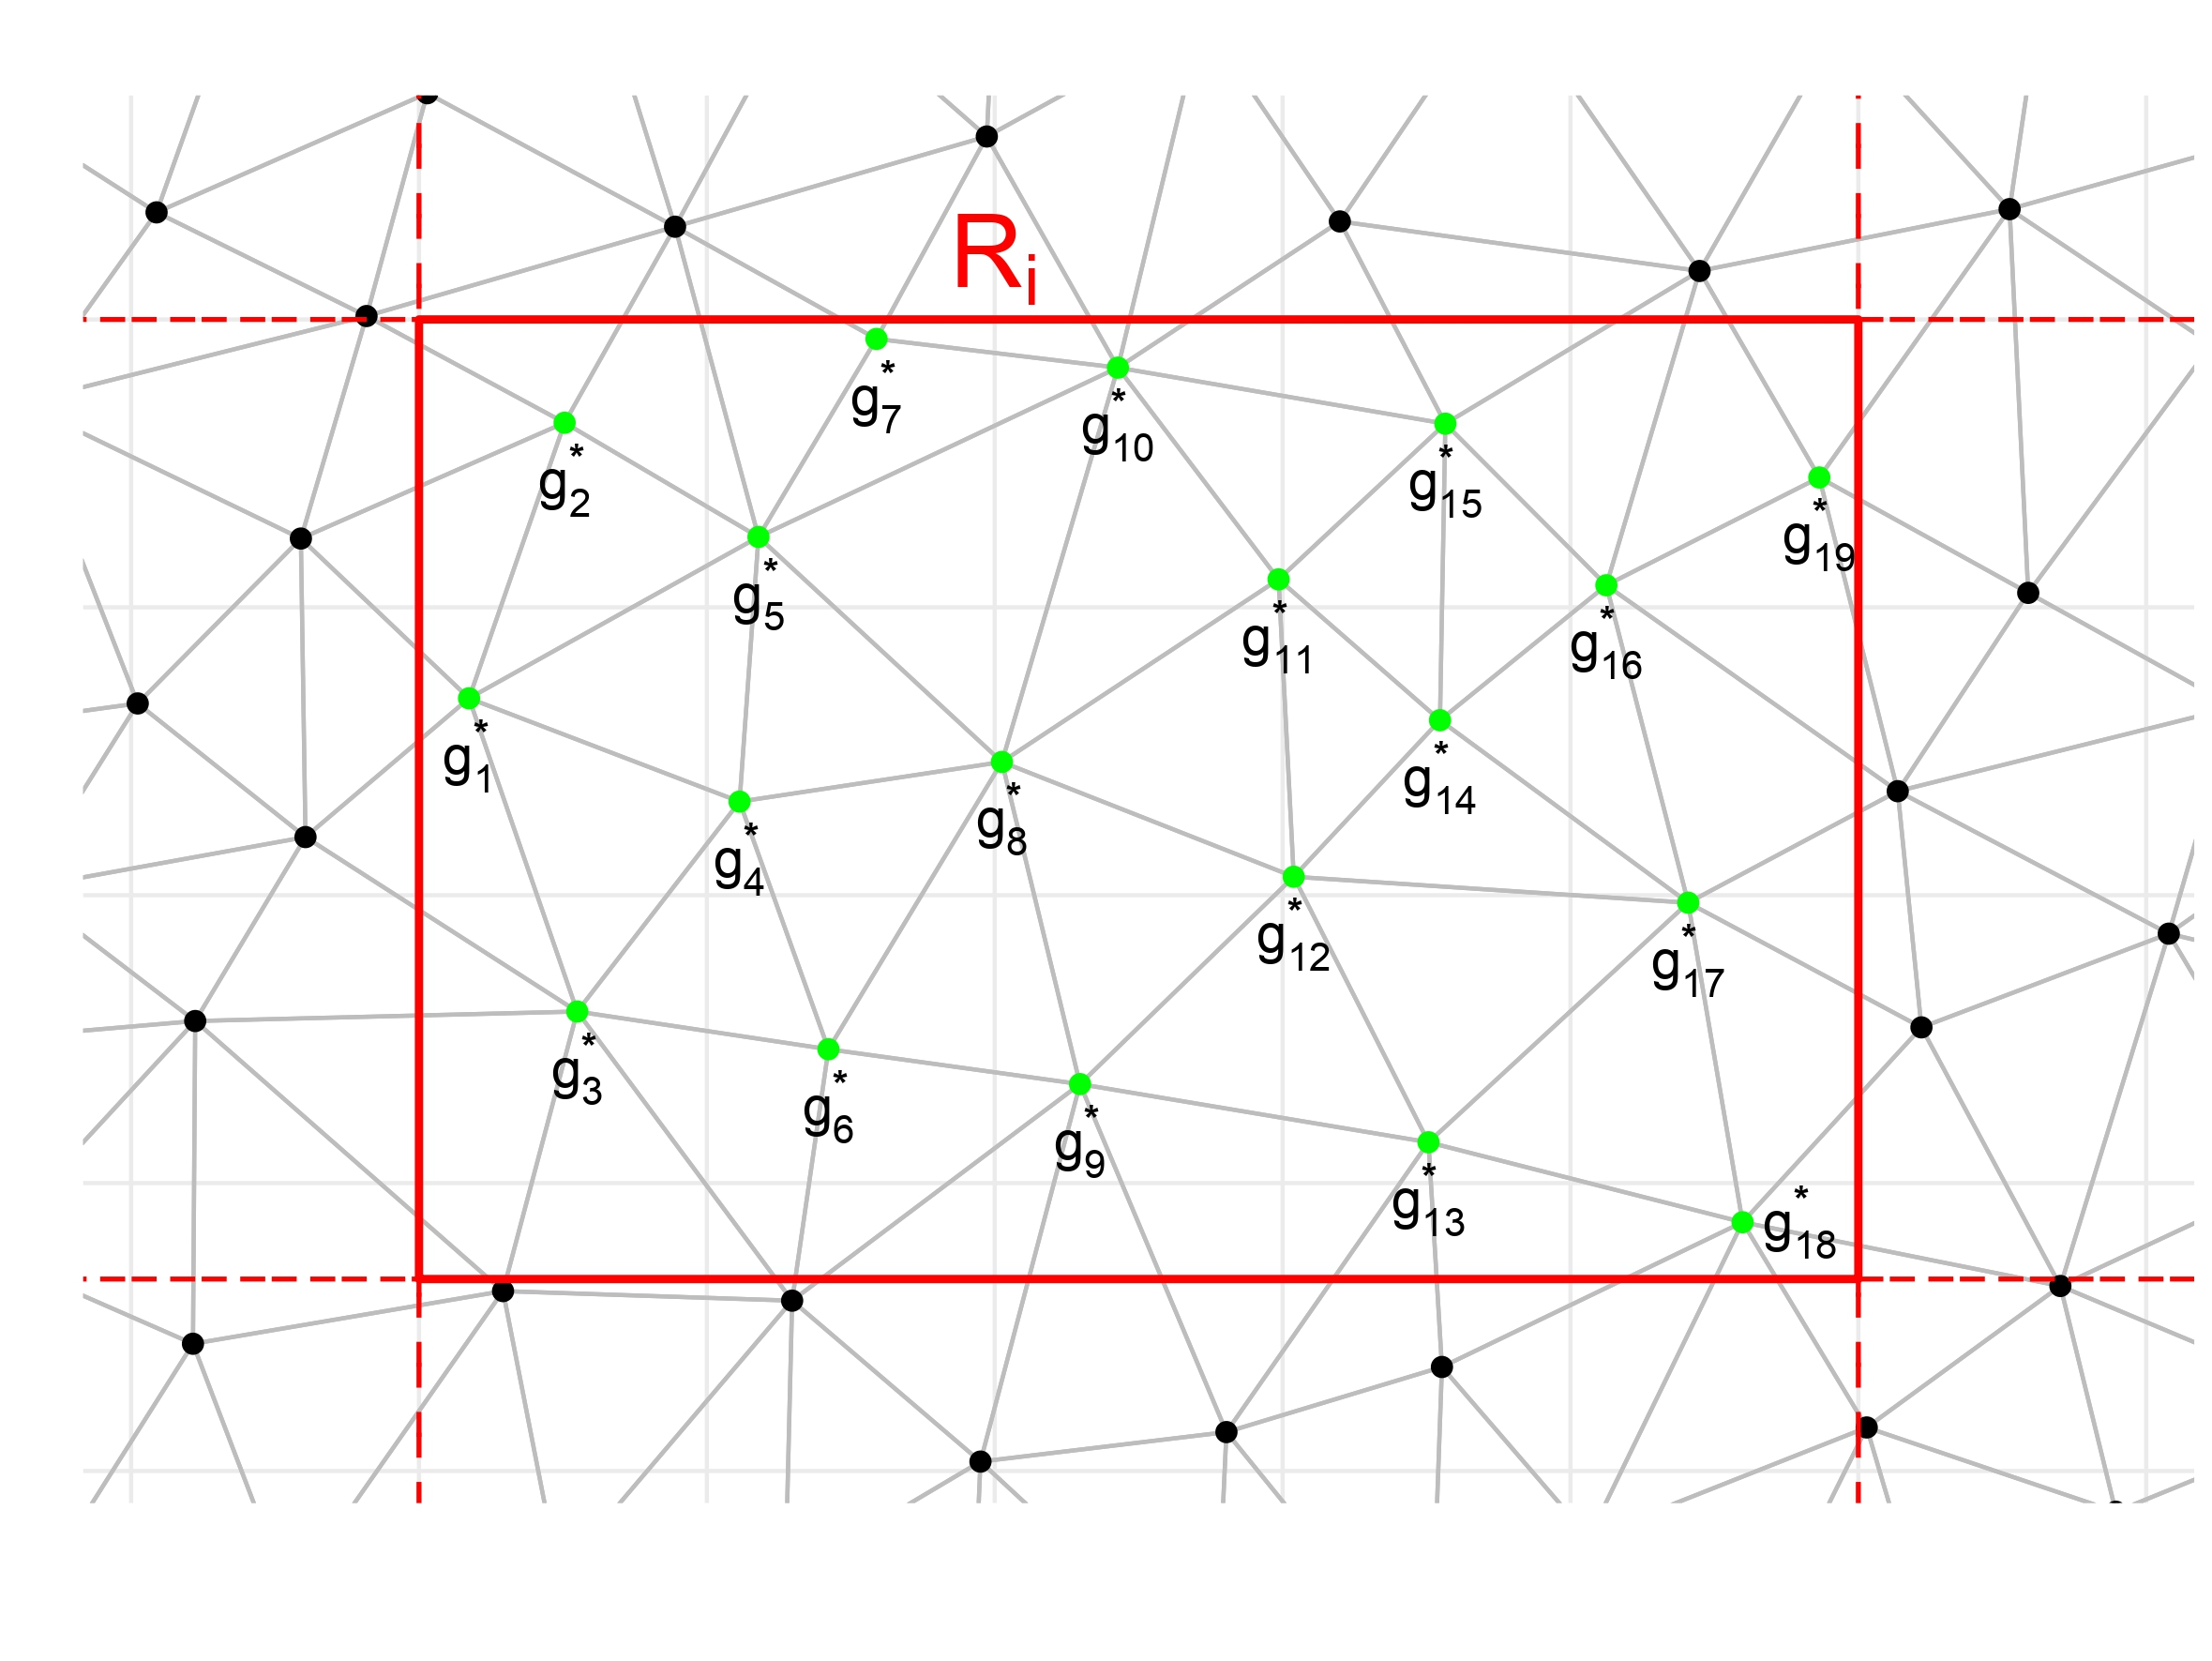
\includegraphics[width=0.6\linewidth]{images/mesh} 

}

\caption{Example of a rectangular region $R_i$ overlaid on a triangulated mesh, where the green vertices are the mesh nodes inside $R_i$ and are used to define the projection matrix A.}\label{fig:mesh-example}
\end{figure}

In \texttt{INLA}, these mappings are implemented by defining the SPDE model on the mesh and supplying the projection matrices in the \texttt{inla.stack()} objects for estimation and prediction.

\subsection{INLA essentials: installation and main workflow}\label{sec:inla-essentials}

Before running the examples in this paper, we need to install \texttt{INLA} and a small set of supporting packages for handling rasters, vector geometries, and meshes. Note that \texttt{INLA} is installed from the INLA repository (not from CRAN).

\begin{verbatim}
# Install INLA from the INLA repository (not CRAN)
install.packages(
  "INLA",
  repos = c(getOption("repos"), INLA = "https://inla.r-inla-download.org/R/stable"),
  dependencies = TRUE
)

# Quick check
library(INLA)
inla.version()
\end{verbatim}

Once the data and covariates are ready, the INLA workflow in this paper follows a fairly standard sequence. First, we build a triangulated mesh to represent the latent field with the SPDE approach. In our examples, the mesh is constructed over the study region using functions such as \texttt{fm\_hexagon\_lattice()} and \texttt{fm\_mesh\_2d()} (from \texttt{fmesher}), choosing parameters like \texttt{max.edge} and \texttt{offset} so the mesh is finer than the original data support.

Next, we define prediction locations on the target resolution, using helpers such as \texttt{st\_make\_grid()}, \texttt{seq()}, and \texttt{expand.grid()}. For the spatio-temporal example, we extend the prediction set by combining the spatial prediction grid with a time index, so the same locations are repeated across the time points where we want predictions. Finally, for both estimation and prediction, the covariates must be available on the same supports as the response. Model specification in INLA is done by translating the linear predictor into a formula and defining the latent SPDE component. The Matérn SPDE is created with \texttt{inla.spde2.matern()}, and the latent field enters the formula through terms like \texttt{f(s,\ model\ =\ spde)}.

To connect the data support (coarse cells) to the mesh representation, we build projection matrices and assemble the stacks. Spatially, the key object is the projection matrix (e.g., \texttt{A.m} from regions to mesh nodes, and \texttt{A.pr} from mesh nodes to prediction points). In practice, we pass these matrices to \texttt{inla.stack()} through its \texttt{A=} argument, and we build separate stacks for estimation and prediction, which are then combined into a single object (e.g., \texttt{stk.full}).

Finally, we fit the model with \texttt{inla()}. The stacked data are provided with \texttt{inla.stack.data()}, and the corresponding projection matrix is passed through \texttt{control.predictor\ =\ list(A\ =\ inla.stack.A(...),\ compute\ =\ TRUE)} so INLA returns fitted values and predictions. Predictions are retrieved using \texttt{inla.stack.index()} to select the prediction rows, and then extracting the posterior summaries from \texttt{res\$summary.linear.predictor}. Fixed-effect summaries are obtained from \texttt{res\$summary.fixed}, and the same workflow extends naturally from the univariate spatial example to the multivariate and spatio-temporal settings by changing the model formula and the stack/projection structure.

\section{Spatial disaggregation of PM2.5 concentration in Portugal}\label{sec:spatial-dis}

In this section, we illustrate spatial disaggregation by improving the resolution of PM2.5 concentrations in Portugal from 10km to 2km. We used annual air quality reanalysis data for Portugal provided by the Copernicus Atmosphere Monitoring Service (CAMS) \citep{inness2019cams}, a high-resolution product developed by the European Centre for Medium-Range Weather Forecasts (ECMWF). This publicly accessible dataset, available at \url{https://ads.atmosphere.copernicus.eu/datasets/cams-europe-air-quality-reanalyses}, integrates satellite observations and auxiliary information to get estimations of air pollution levels in a very corase resolution.

\subsection{PM2.5 disaggregation model}\label{pm2.5-disaggregation-model}

The main objective of this model is to perform spatial disaggregation by increasing the resolution from \(0.1^\circ\) to \(0.02^\circ\), which corresponds approximately to a change from 10 km to 2 km, using \texttt{INLA}. We also include elevation as a high-resolution covariate to help explain local variation in PM2.5 and improve the disaggregation. The model assumes the existence of a latent continuous spatial process for PM2.5 that is observed only through aggregated measurements. Specifically,

\begin{equation}
\text{pm}_{2.5}(\mathbf{s}) = \beta_0 + \beta_1\,\text{elevation}(\mathbf{s}) + z(\mathbf{s}) + e(\mathbf{s}) \label{eq:app-pm25}
\end{equation}
where \(\beta_0\) is an intercept and \(\beta_1\) is the regression coefficient associated with elevation. The term \(z(\mathbf{s})\) represents a spatially structured random effect, modeled as a zero mean Gaussian process with a Mat\textquotesingle ern covariance function, and \(e(\mathbf{s})\) is an unstructured error term, modeled as a zero mean Gaussian process that is independent across space.
The link between the latent field and the areal observations is defined through Equations \eqref{eq:spa-cont}, \eqref{eq:spa-agg}, and \eqref{eq:spa-areal}. Inference is then performed using the projection (aggregation) matrix described in Section \ref{sec:inla-inf-spa}.

\subsection{Data acquisition and preprocessing}\label{sec:spatial-data-pre}

In this section, we describe how to obtain the PM2.5 dataset and the covariate information used in our model. We first show how to download and preprocess the air pollution data, and then we explain how to collect elevation data preprocessing for modeling using \texttt{INLA}.

\subsubsection{Observed PM2.5 values in Portugal}\label{observed-pm2.5-values-in-portugal}

To download PM2.5 data, we need to create an account on the Atmospheric Data Store (ADS), accept the terms and conditions, and obtain the ``Licence to use Copernicus Products.'' After setup, the data can be downloaded using the Python API. More details on setting up the API are available at \url{https://ads.atmosphere.copernicus.eu/how-to-api}. In our request, the argument \texttt{variable\ =\ {[}"particulate\_matter\_2.5um"{]}} selects PM2.5 concentrations, \texttt{model\ =\ {[}"ensemble"{]}} specifies the ensemble product, \texttt{level\ =\ {[}"0"{]}} indicates the surface level, \texttt{type\ =\ {[}"validated\_reanalysis"{]}} requests the validated reanalysis product, and \texttt{year\ =\ {[}"2019"{]}} and \texttt{month\ =\ {[}"01"{]}} restrict the download to January 2019.

After downloading and unzipping the data, we use the \texttt{terra} package to read the \texttt{nc} file. NetCDF (Network Common Data Form) files are widely used for storing multi-dimensional scientific data, such as climate or GIS datasets, because they are self-describing, portable, and efficient for large arrays. The original dataset contains hourly samples for the 31 days of January 2019, totaling 744 observations. Since our focus is on identifying mean trends, we calculated the average PM2.5 concentration for each location. As the original data covers the entire European continent, we cropped the spatial extent to focus specifically on Portugal. To provide better geographical context in our visualizations, we also included the administrative boundaries of Portugal and Spain for clear regional identification using packages \texttt{rnaturalearth} and \texttt{sf}. Finally for plotting we used \texttt{ggplot2}, \texttt{tidyterra} and \texttt{viridis} packages.

\begin{verbatim}
# Define the squared study region
sq <- ext(-9.65, -6.05, 36.85, 42.25)

# Read the dataset and compute mean value (From source)
r <- rast("data/cams.eaq.vra.ENSa.pm2p5.l0.2019-01.nc")
r_mean <- app(r, mean, na.rm = TRUE)
r_sq <- crop(r_mean, sq)
df <- as.data.frame(r_sq, xy = TRUE, na.rm = TRUE)
df <- df[order(df$y, df$x), ]
names(df) <- c("longitude", "latitude", "pm2p5")
write.csv(df, "data/pm2p5_portugal.csv", row.names = FALSE)
\end{verbatim}

To simplify replication and avoid the ADS download and NetCDF preprocessing steps, we provide the preprocessed dataset as \texttt{pm2p5\_portugal.csv}, which contains the processed PM2.5 values in CSV format. Figure (\ref{fig:pm25-plot}) shows the spatial distribution of mean PM2.5 over the Portugal for January 2019. Higher concentrations are observed in northern Portugal. The map is provided on the original CAMS grid (about 0.1\(^\circ\), roughly 10 km), which is relatively coarse for local-scale interpretation; we therefore target a finer resolution of 0.02\(^\circ\) (approximately 2 km) using spatial disaggregation.

\begin{verbatim}
# Define the squared study region
sq <- ext(-9.65, -6.05, 36.85, 42.25)

# Read dataset from preprocess file
df <- read.csv("data/pm2p5_portugal.csv")
r_sq <- rast(df[, c("longitude", "latitude", "pm2p5")])

# Get Portugal and Spain borders
boundary <- ne_countries(scale="medium", returnclass="sf") |>
  subset(admin %in% c("Portugal", "Spain")) |>
  st_transform(4326)

# Plot PM2.5 contamination and boundary countries
ggplot() +
  geom_spatraster(data = r_sq) +
  geom_sf(data = boundary, fill = NA, color = "black") +
  scale_fill_viridis_c(name = "PM2.5") +
  theme(
    axis.text.x = element_text(angle = 45, hjust = 1, vjust = 1, size = 9)
  ) +
  coord_sf(xlim = c(xmin(sq), xmax(sq)),
           ylim = c(ymin(sq), ymax(sq)),
           expand = FALSE)
\end{verbatim}

\begin{figure}

{\centering \includegraphics{my-rjournal-paper_files/figure-latex/pm25-plot-1} 

}

\caption{Mean PM2.5 concentration in Portugal during January 2019. Country boundaries for Portugal and Spain are overlaid for geographic reference.}\label{fig:pm25-plot}
\end{figure}

\subsubsection{Covariates}\label{sec:cov}

We incorporate high resolution elevation data, at approximately \(60\)m resolution, from the EuroDEM product maintained by EuroGeographics \citep{eurogeographics2023eurodem} that is available in the following website \url{https://www.mapsforeurope.org/datasets/euro-dem}. Elevation is included as a covariate to relate PM2.5 concentrations with changes in altitude and to improve the explanatory power of the spatial disaggregation model across the study region. This step can be computationally demanding because EuroDEM is provided at very fine resolution and covers all Europe, and it must be reprojected to EPSG:4326 before cropping. To reduce computation time, we provide a preprocessed version already reprojected, aggregated and cropped to the study region called \texttt{eurodemc.tif}.

\begin{verbatim}
# Time consuming: This preprocessing takes roughly 40 minutes to be executed
r <- rast("data/eurodem.tif")
r_map <- project(r, "EPSG:4326")
writeRaster(r_map, "data/eurodemp.tif", overwrite = TRUE)
r_map <- rast("data/eurodemp.tif")
r_crop <- crop(r_map, sq_sf)
r_ag <- aggregate(r_crop, fact = 2, fun = mean, na.rm = TRUE)
writeRaster(r_ag, "data/eurodemc.tif", overwrite = TRUE)
\end{verbatim}

After preprocessing, Figure (\ref{fig:elev-plot-1}) shows the resulting elevation raster over Portugal, with values reported in meters.

\begin{verbatim}
# Reading elevation dataset
r_crop <- rast("data/eurodemc.tif")
r_crop[is.na(r_crop)] <- 0

plot(r_crop)
\end{verbatim}

\begin{figure}

{\centering \includegraphics{my-rjournal-paper_files/figure-latex/elev-plot-1-1} 

}

\caption{EuroDEM elevation raster over Portugal (meters), cropped to the study region and used as a covariate in the disaggregation model.}\label{fig:elev-plot-1}
\end{figure}

\subsection{INLA modeling}\label{inla-modeling}

After obtaining the PM2.5 dataset and the elevation covariate, we need to prepare several additional objects before fitting the disaggregation model with \texttt{INLA}. We proceed in the following order. First, we define the input grid, build the spatial mesh, and create the prediction locations on the finer resolution grid. Next, we align the elevation covariate with both the input grid and the prediction grid. We then specify the SPDE in the spatial mesh, construct the projection matrices and assemble the corresponding \texttt{INLA} stacks for estimation and prediction. Finally, we fit the model with \texttt{INLA} and summarize the results, and we compare the coarse input field with the disaggregated predictions on the finer scale.

\subsubsection{Input grid, mesh, and prediction locations}\label{sec:mesh}

The first step in the disaggregation workflow is to construct an input grid that matches the support of the observed data. Using the dataframe \texttt{df}, we build a squared grid as an \texttt{sf} object with the same spatial extent and dimensions as the original dataset. The second step is to build a spatial mesh that is finer than the initial resolution of the data, as shown on the right side of Figure (\ref{fig:mesh-plot}). This panel displays a portion of the triangulated mesh, represented by black segments, together with the original gridded support, shown in red. Finally, to achieve the target disaggregation from 0.1\(^\circ\) to 0.02\(^\circ\), we define the prediction points on the desired high resolution grid. The variable \texttt{spf} controls the disaggregation factor. Specifically, setting \(\texttt{spf}=5\) increases the resolution within each original cell by a factor of \(5 \times 5 = 25\), as illustrated on the left side of Figure (\ref{fig:mesh-plot}), where red lines denote the original grid and blue dots indicate the prediction locations under the disaggregated scenario.

\begin{verbatim}
# Initial squared grid
map <- st_as_sf(st_make_grid(sq, n = c(length(unique(df$longitude)),
                               length(unique(df$latitude)))))
st_geometry(map) <- "geometry"
st_crs(map) <- "EPSG:4326"

# Spatial mesh
sq_sf <- st_as_sf(as.polygons(sq))

hexpts <- fm_hexagon_lattice(
  bnd = st_buffer(sq_sf, 0.1),
  edge_len = 0.05
)

mesh <- fm_mesh_2d(
  loc = hexpts,
  max.edge = 0.1,
  offset = 0.05
)

# prediction points

spf <- 5 # spatial factor
def <- abs(unique(df$latitude)[2]-unique(df$latitude)[1])/2

x <- seq(min(df$longitude) - def*((spf-1)/spf),
         max(df$longitude) + def*((spf-1)/spf),
         length.out = length(unique(df$longitude))*spf)

y <- seq(min(df$latitude) - def*((spf-1)/spf),
         max(df$latitude) + def*((spf-1)/spf),
         length.out = length(unique(df$latitude))*spf)

dp <- as.matrix(expand.grid(x, y))
dpdf <- data.frame(dp)
names(dpdf) <- c("x", "y")

dpdf_sf <- st_as_sf(dpdf, coords = c("x", "y"), crs="EPSG:4326")
dpdf_sf$id <- 1:nrow(dpdf)

# Plots
par(mfrow = c(1, 2), pty = "s")
plot(mesh, xlim = c(-9.65, -9.45), ylim = c(36.5, 37.5))
plot(map$geometry, add = TRUE, border = "red", lwd = 2)

plot(map$geometry, border = "red", lwd = 2 , xlim = c(-9.7, -9.5),
     ylim = c(36.8, 37))
plot(dpdf_sf$geometry, add = TRUE, col = "blue", lwd = 1)
\end{verbatim}

\begin{figure}

{\centering \includegraphics{my-rjournal-paper_files/figure-latex/mesh-plot-1} 

}

\caption{Spatial discretization for disaggregation. Original grid support is shown in red. Prediction points for `spf=5` are shown in blue (left), and a portion of the triangulated mesh is shown in black (right)}\label{fig:mesh-plot}
\end{figure}

\subsubsection{Elevation covariate on input and prediction grids}\label{elevation-covariate-on-input-and-prediction-grids}

To incorporate this covariate within the disaggregation framework, we align its spatial support with both the original CAMS grid and the high-resolution prediction grid. For this purpose, we use the \texttt{exactextractr} package, which provides efficient tools for extracting and summarizing raster values over polygonal features. We compute the mean elevation within each 0.1\(^\circ\) CAMS input cell and within each 0.02\(^\circ\) prediction cell, so that the covariate is available at the same spatial support as both the observed and predicted quantities. Figure (\ref{fig:elev-plot-2}) illustrates the resulting elevation covariate over Portugal, with the input grid shown on the left and the prediction grid shown on the right.

\begin{verbatim}
# Time consuming: this part takes around 1 minute to be executed
# Converting to Raster* object
r_ras <- raster::raster(r_crop)

# Extract elevation values in the original dataset
map$elev <- exact_extract(r_ras, map, "mean", progress = FALSE)

# Create the prediction dataset in sf format
map_pred <- st_as_sf(st_make_grid(sq, n = c(length(unique(df$longitude)),
                               length(unique(df$latitude)))*spf))
st_crs(map_pred) <- "EPSG:4326"

# Extract elevation values in the prediction dataset
map_pred$elev <- exact_extract(r_ras, map_pred, "mean", progress = FALSE)

# Plot elevation in the input grid
p1 <- ggplot(map) +
  geom_sf(aes(fill = elev), color = NA) +
  scale_fill_viridis_c(name = "Elevation (m)") +
  geom_sf(data = boundary, fill = NA, color = "black") +
  coord_sf(xlim = c(-10, -6), ylim = c(36.5, 42.5),
           expand = FALSE) +
  theme(
    axis.text.x = element_text(angle = 45, hjust = 1, vjust = 1, size = 9),
    plot.margin = margin(t = 5.5, r = 5.5, b = 18, l = 5.5)
  )

# Plot elevation in the prediction grid
p2 <- ggplot(map_pred) +
  geom_sf(aes(fill = elev), color = NA) +
  scale_fill_viridis_c(name = "Elevation (m)") +
  geom_sf(data = boundary, fill = NA, color = "black") +
  coord_sf(xlim = c(-10, -6), ylim = c(36.5, 42.5),
           expand = FALSE) +
  theme(
    axis.text.x = element_text(angle = 45, hjust = 1, vjust = 1, size = 9),
    plot.margin = margin(t = 5.5, r = 5.5, b = 18, l = 5.5)
  )

p1 + p2
\end{verbatim}

\begin{figure}

{\centering \includegraphics{my-rjournal-paper_files/figure-latex/elev-plot-2-1} 

}

\caption{Elevation over Portugal on the input grid (left) and the prediction grid (right), with country boundaries for reference.}\label{fig:elev-plot-2}
\end{figure}

\subsubsection{SPDE especification, projection matrices and INLA stacks}\label{sec:mod-inp}

To fit the model described in Equation \eqref{eq:app-pm25}, we use the triangulated mesh defined before in Section \ref{sec:mesh}. We then construct the SPDE representation on this mesh, and build the corresponding projection matrices that link the observation locations and the prediction points to the mesh nodes. Finally, we combine the response, covariates, and latent components into \texttt{INLA} stacks, which are used to perform model estimation and prediction.

\begin{verbatim}
# Construct the SPDE in the spatial mesh
spde <- inla.spde2.matern(mesh = mesh, alpha = 2, constr = TRUE)

n.ar <- nrow(map) # number of initial regions
nv <- mesh$n # number of mesh nodes

mesh_sf <- st_as_sf(data.frame(x=mesh$loc[, 1], y=mesh$loc[, 2], id=1:nv),
                    coords = c("x", "y"), crs="EPSG:4326")

# Projection matrix from initial data to the triangulated mesh
A.m <- matrix(0, n.ar, nv)
inter <- as.list(st_contains(map[, c()], mesh_sf))

for (i in 1:n.ar){
  idx <- inter[[i]]
  A.m[i, idx] <- 1/length(idx)
}
A.m <- as(A.m, "dgCMatrix")

# Projection matrix from the mesh to the predicted points
A.pr <- inla.spde.make.A(mesh = mesh, loc = dp)

# Stack for estimation
stk.est <- inla.stack(
  data = list(y = df$pm2p5),
  A = list(A.m, A.m, 1),
  effects = list(
    s = 1:nv,
    b0 = rep(1, nv),
    elev = map$elev/1000 # convert m to km
  ),
  tag = "y")

# Stack for prediction
stk.pred <- inla.stack(
  data = list(y = NA),
  A = list(A.pr, A.pr, 1),
  effects = list(
    s = 1:nv,
    b0 = rep(1, nv),
    elev = map_pred$elev/1000 # convert m to km
    ),
  tag = "y.pred")

# Stack for estimation and prediction
stk.full <- inla.stack(stk.est, stk.pred)
\end{verbatim}

\subsubsection{Model fitting with INLA}\label{model-fitting-with-inla}

Now, we translate Equation \eqref{eq:app-pm25} into an \texttt{INLA} formula, where the symbol \texttt{\textasciitilde{}} defines the linear predictor for the response \(y\). The term \texttt{0\ +\ b0} adds an explicit intercept, with \texttt{b0} being a column of ones included in the stack. The term \texttt{elev} represents elevation as a fixed effect, and \texttt{f(s,\ model\ =\ spde)} specifies the spatial random effect on the mesh using the SPDE model. We fit the model with \texttt{inla()} using the stacked data object \texttt{stk.full}, and set \texttt{family\ =\ "gaussian"} because \(y\) is continuous.

\begin{verbatim}
# Time consuming: This preprocessing takes roughly 5 minutes to be executed

# INLA formula
form <- y ~ 0 + b0 + elev + f(s, model = spde)

# Fitting and prediction
res <- inla(
  formula=form,
  data = inla.stack.data(stk.full, spde = spde),
  family = "gaussian",
  control.predictor = list(A = inla.stack.A(stk.full),
                           compute = TRUE, link = 1)
)

# Summary for the fixed effects
res$summary.fixed |>
  knitr::kable(digits = 3) |>
  kable_styling(full_width = FALSE)
\end{verbatim}

\begin{table}
\centering
\caption{\label{tab:fixed-table}Posterior summary of the fixed effects (intercept and elevation coefficient) for the PM2.5 concentration model in Portugal.}
\centering
\begin{tabular}[t]{l|r|r|r|r|r|r|r}
\hline
  & mean & sd & 0.025quant & 0.5quant & 0.975quant & mode & kld\\
\hline
b0 & 8.345 & 0.022 & 8.303 & 8.345 & 8.387 & 8.345 & 0\\
\hline
elev & -0.439 & 0.073 & -0.582 & -0.439 & -0.297 & -0.439 & 0\\
\hline
\end{tabular}
\end{table}

Table (\ref{tab:fixed-table}) summarizes the posterior distributions of the fixed effects. The posterior mean of the intercept \(\beta_0\) is 8.34 \(\mu\)g/m\(^3\), which represents the mean PM2.5 level over Portugal when elevation is zero. The posterior credible interval for the elevation coefficient excludes zero, indicating a clear association between elevation and PM2.5. The posterior mean is \(-0.44\), implying that an increase of 1 km in altitude is associated with a decrease of about 0.44 \(\mu\)g/m\(^3\) in PM2.5.

\subsubsection{Input data and disaggregated predictions}\label{input-data-and-disaggregated-predictions}

Figure (\ref{fig:pred-plot}) compares the coarse input PM2.5 field (left) with the posterior mean predictions from the disaggregation model on the finer grid (right). The disaggregated surface provides a smoother and more detailed representation of spatial variability, while maintaining the main concentration levels and spatial patterns observed in the input data.We also notice that the range of the predicted surface is slightly wider than the range of the input data. This is an important advantage of the disaggregation approach, since it can reveal localized areas with higher or lower concentrations than suggested by the coarse grid, which can be useful for decision-makers.

\begin{verbatim}
# get indexes of the response variable
idx <- inla.stack.index(stk.full, 'y.pred')$data

# Input grid
map$pm2p5 <- df$pm2p5

# Prediction
map_pred$pm2p5 <- res$summary.linear.predictor[idx, "mean"]

# Plot for input grid
p1 <- ggplot(map) +
  geom_sf(aes(fill = pm2p5), color = NA) +
  scale_fill_viridis_c(name = "Pm2.5") +
  geom_sf(data = boundary, fill = NA, color = "black") +
  coord_sf(xlim = c(-10, -6), ylim = c(36.5, 42.5),
           expand = FALSE) +
  theme(
    axis.text.x = element_text(angle = 45, hjust = 1, vjust = 1, size = 9),
    plot.margin = margin(t = 5.5, r = 5.5, b = 18, l = 5.5)
  )

# Plot for predictions
p2 <- ggplot(map_pred) +
  geom_sf(aes(fill = pm2p5), color = NA) +
  scale_fill_viridis_c(name = "Pm2.5") +
  geom_sf(data = boundary, fill = NA, color = "black") +
  coord_sf(xlim = c(-10, -6), ylim = c(36.5, 42.5),
           expand = FALSE) +
  theme(
    axis.text.x = element_text(angle = 45, hjust = 1, vjust = 1, size = 9),
    plot.margin = margin(t = 5.5, r = 5.5, b = 18, l = 5.5)
  )

# Combine plots
p1 + p2
\end{verbatim}

\begin{figure}

{\centering \includegraphics{my-rjournal-paper_files/figure-latex/pred-plot-1} 

}

\caption{PM2.5 over Portugal on the input grid (left) and disaggregated predictions on the finer grid (right).}\label{fig:pred-plot}
\end{figure}

Within this framework, covariates are incorporated at the fine scale, allowing high-resolution information to capture local variation that would otherwise be obscured at coarser supports. A central practical component is the projection matrix, which links the mesh-based representation of the latent field to the observed spatial units.

By adopting the INLA--SPDE approach, the latent field is represented on a triangulated mesh (and extended to a spatio-temporal mesh when needed), enabling computationally efficient inference while retaining full Bayesian uncertainty quantification.

\section{Conclusion and discussion}\label{sec:con}

In this paper we have demonstrated how to perform spatial disaggregation with \texttt{INLA}.Using an application to PM2.5 data, we have shown how to formulate a spatial disaggregation model by assuming an underlying latent Gaussian field defined at a finer scale than the observed data. The observations are then treated as aggregated measurements of this latent field over larger spatial units. Within this framework, covariates are incorporated at the fine scale, allowing high-resolution information to capture local variation that would otherwise be obscured at coarser supports. The key practical component in the implementation is the projection matrix, which links the mesh representation of the latent field to the observed spatial units. By adopting the INLA--SPDE approach, we represent the latent field on a triangulated mesh which makes inference computationally efficient while still providing full Bayesian uncertainty quantification.

In the application presented, we disaggregate PM2.5 over Portugal from the CAMS \(0.1^\circ\) grid to \(0.02^\circ\), and we include elevation (EuroDEM) as a covariate to relate pollution levels to altitude and improve the spatial interpretation.This framework is based on the implementation developed in \citep{moraga2017geostatistical}. This approach can be extended to multivariate settings by jointly disaggregating several air pollutants, and spatio-temporal settings to estimate variables at higher resolutions both in space in time.For example, \citep{RodriguezAvellanedaMult} utilized a multivariate setting using the Linear Model of Coregionalization (LMC), to jointly disaggregate PM2.5, PM10, and ozone over Portugal using the same CAMS product \citep{inness2019cams}.
\citep{avellaneda2025bayesianspatiotemporaldisaggregationmodeling} extended this approach to the spatio-temporal setting and disaggregated Aerosol Optical Depth (AOD) at 550 nm over India using the EAC4 reanalysis from ECMWF \citep{inness2019cams}. In that example, they refined the spatial resolution from \(0.75^\circ\) to \(0.25^\circ\) and the temporal resolution from 3-hourly to hourly, producing spatio-temporal predictions at intermediate time points that were not available in the original product.

The spatial model presented in this paper considers Gaussian responses. A natural extension is to develop spatial disaggregation models for non-Gaussian data, for example Poisson or Binomial outcomes such as disease counts over administrative units. On the spatio-temporal side, recent work has proposed efficient spatial disaggregation methods for spatio-temporal datasets \citep{gaedke2025acceleratedspatiotemporalbayesianmodeling}, while the spatio-temporal model in \citep{avellaneda2025bayesianspatiotemporaldisaggregationmodeling} goes one step further by disaggregating not only in space but also in time. A further direction is to combine these ideas and build multivariate spatio-temporal disaggregation models that jointly downscale multiple variables across space and time, and that can handle variables observed on different spatial or temporal supports within a single coherent framework \citep{zhongetal25}.

Overall, this paper presents a practical disaggregation workflow based on latent Gaussian fields and the INLA--SPDE framework, which scales well and can be adapted to spatial, multivariate, and spatio-temporal settings. Although we focus on an air pollution application, the same framework applies to other continuous variables observed on coarse spatial supports, where the goal is to recover the underlying process at a finer resolution with uncertainty quantification. Examples include remotely sensed or reanalysis products such as land-surface temperature, precipitation, soil moisture, sea-surface temperature, and vegetation indices, as well as other environmental exposures available as gridded averages \citep{moragaandbaker22, forlani2020joint, gomez2019multivariate}.

\bibliography{RJreferences.bib,packages.bib}

\address{%
Fernando Rodriguez Avellaneda\\
King Abdullah University of Science and Technology (KAUST)\\%
Thuwal, Saudi Arabia\\
%
\url{https://linkedin.com/in/fr-avellaneda}\\%
\textit{ORCiD: \href{https://orcid.org/0009-0000-0937-0698}{0009-0000-0937-0698}}\\%
\href{mailto:fernando.rodriguezavellaneda@kaust.edu.sa}{\nolinkurl{fernando.rodriguezavellaneda@kaust.edu.sa}}%
}

\address{%
Paula Moraga\\
King Abdullah University of Science and Technology (KAUST)\\%
Thuwal, Saudi Arabia.\\
%
\url{https://www.paulamoraga.com/}\\%
\textit{ORCiD: \href{https://orcid.org/0000-0001-5266-0201}{0000-0001-5266-0201}}\\%
\href{mailto:paula.moraga@kaust.edu.sa}{\nolinkurl{paula.moraga@kaust.edu.sa}}%
}
